\documentclass[Handouts]{beamer} % "Beamer" is a word used in Germany to mean video projector. 

%\usetheme{Warsaw}
%\usetheme{Antibes}
%\usetheme{Bergen}
%\usetheme{Berkeley}
%\usetheme{Berlin}
%\usetheme{Copenhagen}
%\usetheme{Darmstadt}
%\usetheme{Dresden}
%\usetheme{Frankfurt}
%\usetheme{Goettingen}
%\usetheme{Hannover}
%\usetheme{Ilmenau}
%\usetheme{JuanLesPins}
%\usetheme{Luebeck}
%\usetheme{Madrid}
%\usetheme{Malmoe}
%\usetheme{Marburg}
%\usetheme{Montpellier}
%\usetheme{PaloAlto}
%\usetheme{Pittsburgh}
%\usetheme{Rochester}
%\usetheme{Singapore}
%\usetheme{Szeged}
%\usetheme{boxes}
%\usetheme{default}
\usetheme{CambridgeUS}
% Search online for beamer themes to find your favorite or use the Berkeley theme as in this file.

%\usecolortheme{beaver}
%\usecolortheme{default}
%\usecolortheme{albatross}
%\usecolortheme{crane}
%\usecolortheme{dolphin}
%\usecolortheme{dove}
%\usecolortheme{fly}
%\usecolortheme{lily}
%\usecolortheme{orchid}
%\usecolortheme{rose}
%\usecolortheme{seagull}
%\usecolortheme{seahorse}
%\usecolortheme{whale}
%\usecolortheme{wolverine}



\usepackage{color} % It may be necessary to set PCTeX or whatever program you are using to output a .pdf instead of a .dvi file in order to see color on your screen.
\usepackage{graphicx} % This package is needed if you wish to include external image files.
\usepackage{url}
\usepackage{amsmath}
\usepackage{mathrsfs}
%\usepackage{minted}
%\usepackage{media9}
%\usepackage{listings}

%\lstset{ %
%	backgroundcolor=\color{white},   % choose the background color; you must add \usepackage{color} or \usepackage{xcolor}
%	basicstyle=\footnotesize,        % the size of the fonts that are used for the code
%	breakatwhitespace=false,         % sets if automatic breaks should only happen at whitespace
%	breaklines=true,                 % sets automatic line breaking
%	captionpos=b,                    % sets the caption-position to bottom
%	commentstyle=\color{mygreen},    % comment style
%	deletekeywords={...},            % if you want to delete keywords from the given language
%	escapeinside={\%*}{*)},          % if you want to add LaTeX within your code
%	extendedchars=true,              % lets you use non-ASCII characters; for 8-bits encodings only, does not work with UTF-8
%	frame=single,                    % adds a frame around the code
%	keepspaces=true,                 % keeps spaces in text, useful for keeping indentation of code (possibly needs columns=flexible)
%	keywordstyle=\color{blue},       % keyword style
%	language=python,                 % the language of the code
%	morekeywords={*,...},            % if you want to add more keywords to the set
%numbers=left,                    % where to put the line-numbers; possible values are (none, left, right)
%	numbersep=5pt,                   % how far the line-numbers are from the code
%	numberstyle=\tiny\color{mygray}, % the style that is used for the line-numbers
%	rulecolor=\color{black},         % if not set, the frame-color may be changed on line-breaks within not-black text (e.g. comments (green here))
%	showspaces=false,                % show spaces everywhere adding particular underscores; it overrides 'showstringspaces'
%	showstringspaces=false,          % underline spaces within strings only
%	showtabs=false,                  % show tabs within strings adding particular underscores
%	stepnumber=1,                    % the step between two line-numbers. If it's 1, each line will be numbered
%	stringstyle=\color{mymauve},     % string literal style
%	tabsize=2,                       % sets default tabsize to 2 spaces
%	title=\lstname                   % show the filename of files included with \lstinputlisting; also try caption instead of title
%}




\title{IoT with python and RPi}
\author{Dr. Sandeep Nagar} 
%\institute{G. D. Goenka University}
\date{\today} 

\begin{document}
\begin{frame}{IoT}

\centering
\Large{IoT with python and Raspberry Pi}\\
\textbf{PyDelhi 2016}
	
\end{frame}

\begin{frame}{Instructor}
	\begin{figure}
		\centering
		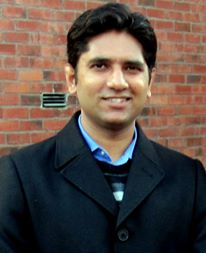
\includegraphics[width=4cm,height=4cm,keepaspectratio]{me}
	\end{figure}
	
	\centering
	\textcolor{blue}{Dr. Sandeep Nagar} \\
	M.Sc. Physics (MSU, Vadodara) \& PhD in Material Science \\ (Department of Material Science and Engineering, KTH, Sweden) \\
	contact e-mail: \textcolor{red}{sandeep.nagar@gmail.com}
\end{frame}

\begin{frame}{Why would I do IoT?}
	\begin{itemize}
		\item Its for everybody!
		\item Started just for fun
		\item Some serious experimentation
		\item Making scientific instruments
		\item Internet control gives multi-functionality to experiments
	\end{itemize}
\end{frame}

\begin{frame}{Outline of workshop}
	\begin{enumerate}
		\item Introduction to IoT and Raspberry Pi ($30$ Minutes)
		\begin{itemize}
			\item Intro to IoT
			\item Various parts
			\item Installing OS
		\end{itemize}
		\item Accessing GPIO pins ($30$ minutes)
		\begin{itemize}
			\item Writing to GPIO pins
			\item Reading from GPIO pins
		\end{itemize}
		\item IoT with RPi ($30$ minutes)
		\begin{itemize}
			\item Running RPi headless 
			\item Adding sensors
			\item Interacting with data generated using IoT device
		\end{itemize}
	\end{enumerate}
\end{frame}

\section{Intro to IoT}

\begin{frame}{Introduction to IoT}
	\begin{itemize}
		\item IoT is a connecting \textbf{things} to internet
		\item Two types:
		\begin{itemize}
			\item Device computes locally and interacts on internet
			\item Device does not compute locally but interacts on internet
		\end{itemize}
		\item Interaction on internet means:
		\begin{itemize}
			\item Write and read data
			\item Write and read code to control systems
		\end{itemize}
	\end{itemize}
\end{frame}

\begin{frame}{Intro to RPi}
	\begin{itemize}
		\item Microcomputer
		\begin{itemize}
			\item Credit card sized ($20 \times 10$ cm)
			\item Weight = $68$ g
		\end{itemize}
		\item Very cost effective
		\begin{itemize}
			\item Presently available for INR $2,875$ at amazon 
		\end{itemize}
		\item Low power consumption 
		\begin{itemize}
			\item We will use mobile phone charger
		\end{itemize}
		\item Remote access over internet
		\begin{itemize}
			\item We will use a LAN cable for connectivity
		\end{itemize}
		\item Runs Linux
		\begin{itemize}
			\item Raspbian is a version of Debian optimized for RPi
		\end{itemize}
	\end{itemize}
\end{frame}

\begin{frame}{Powerful IoT platform}
	\begin{itemize}
		\item Broadcom $900$ MHz BCM$2836$ ARMv$7$ Quad Core Processor SoC 
		\item Broadcom VideoCore IV GPU
		\item $1$ GB RAM
		\item Expanded $40$-pin GPIO Header
		\item $4$ x USB$2.0$ Ports with up to $1.2$A output
		\item $4$ pole Stereo output and Composite video port
		\item Full size HDMI
		\item CSI camera port for connecting the Raspberry Pi camera
		\item DSI display port for connecting the Raspberry Pi touch screen display
		\item Micro SD port for loading your operating system and storing data
		\item Micro USB power source
	\end{itemize}
	Ref: \url{https://www.raspberrypi.org/products/raspberry-pi-2-model-b/}
\end{frame}

\begin{frame}{RPi}
	\begin{figure}
		\centering
		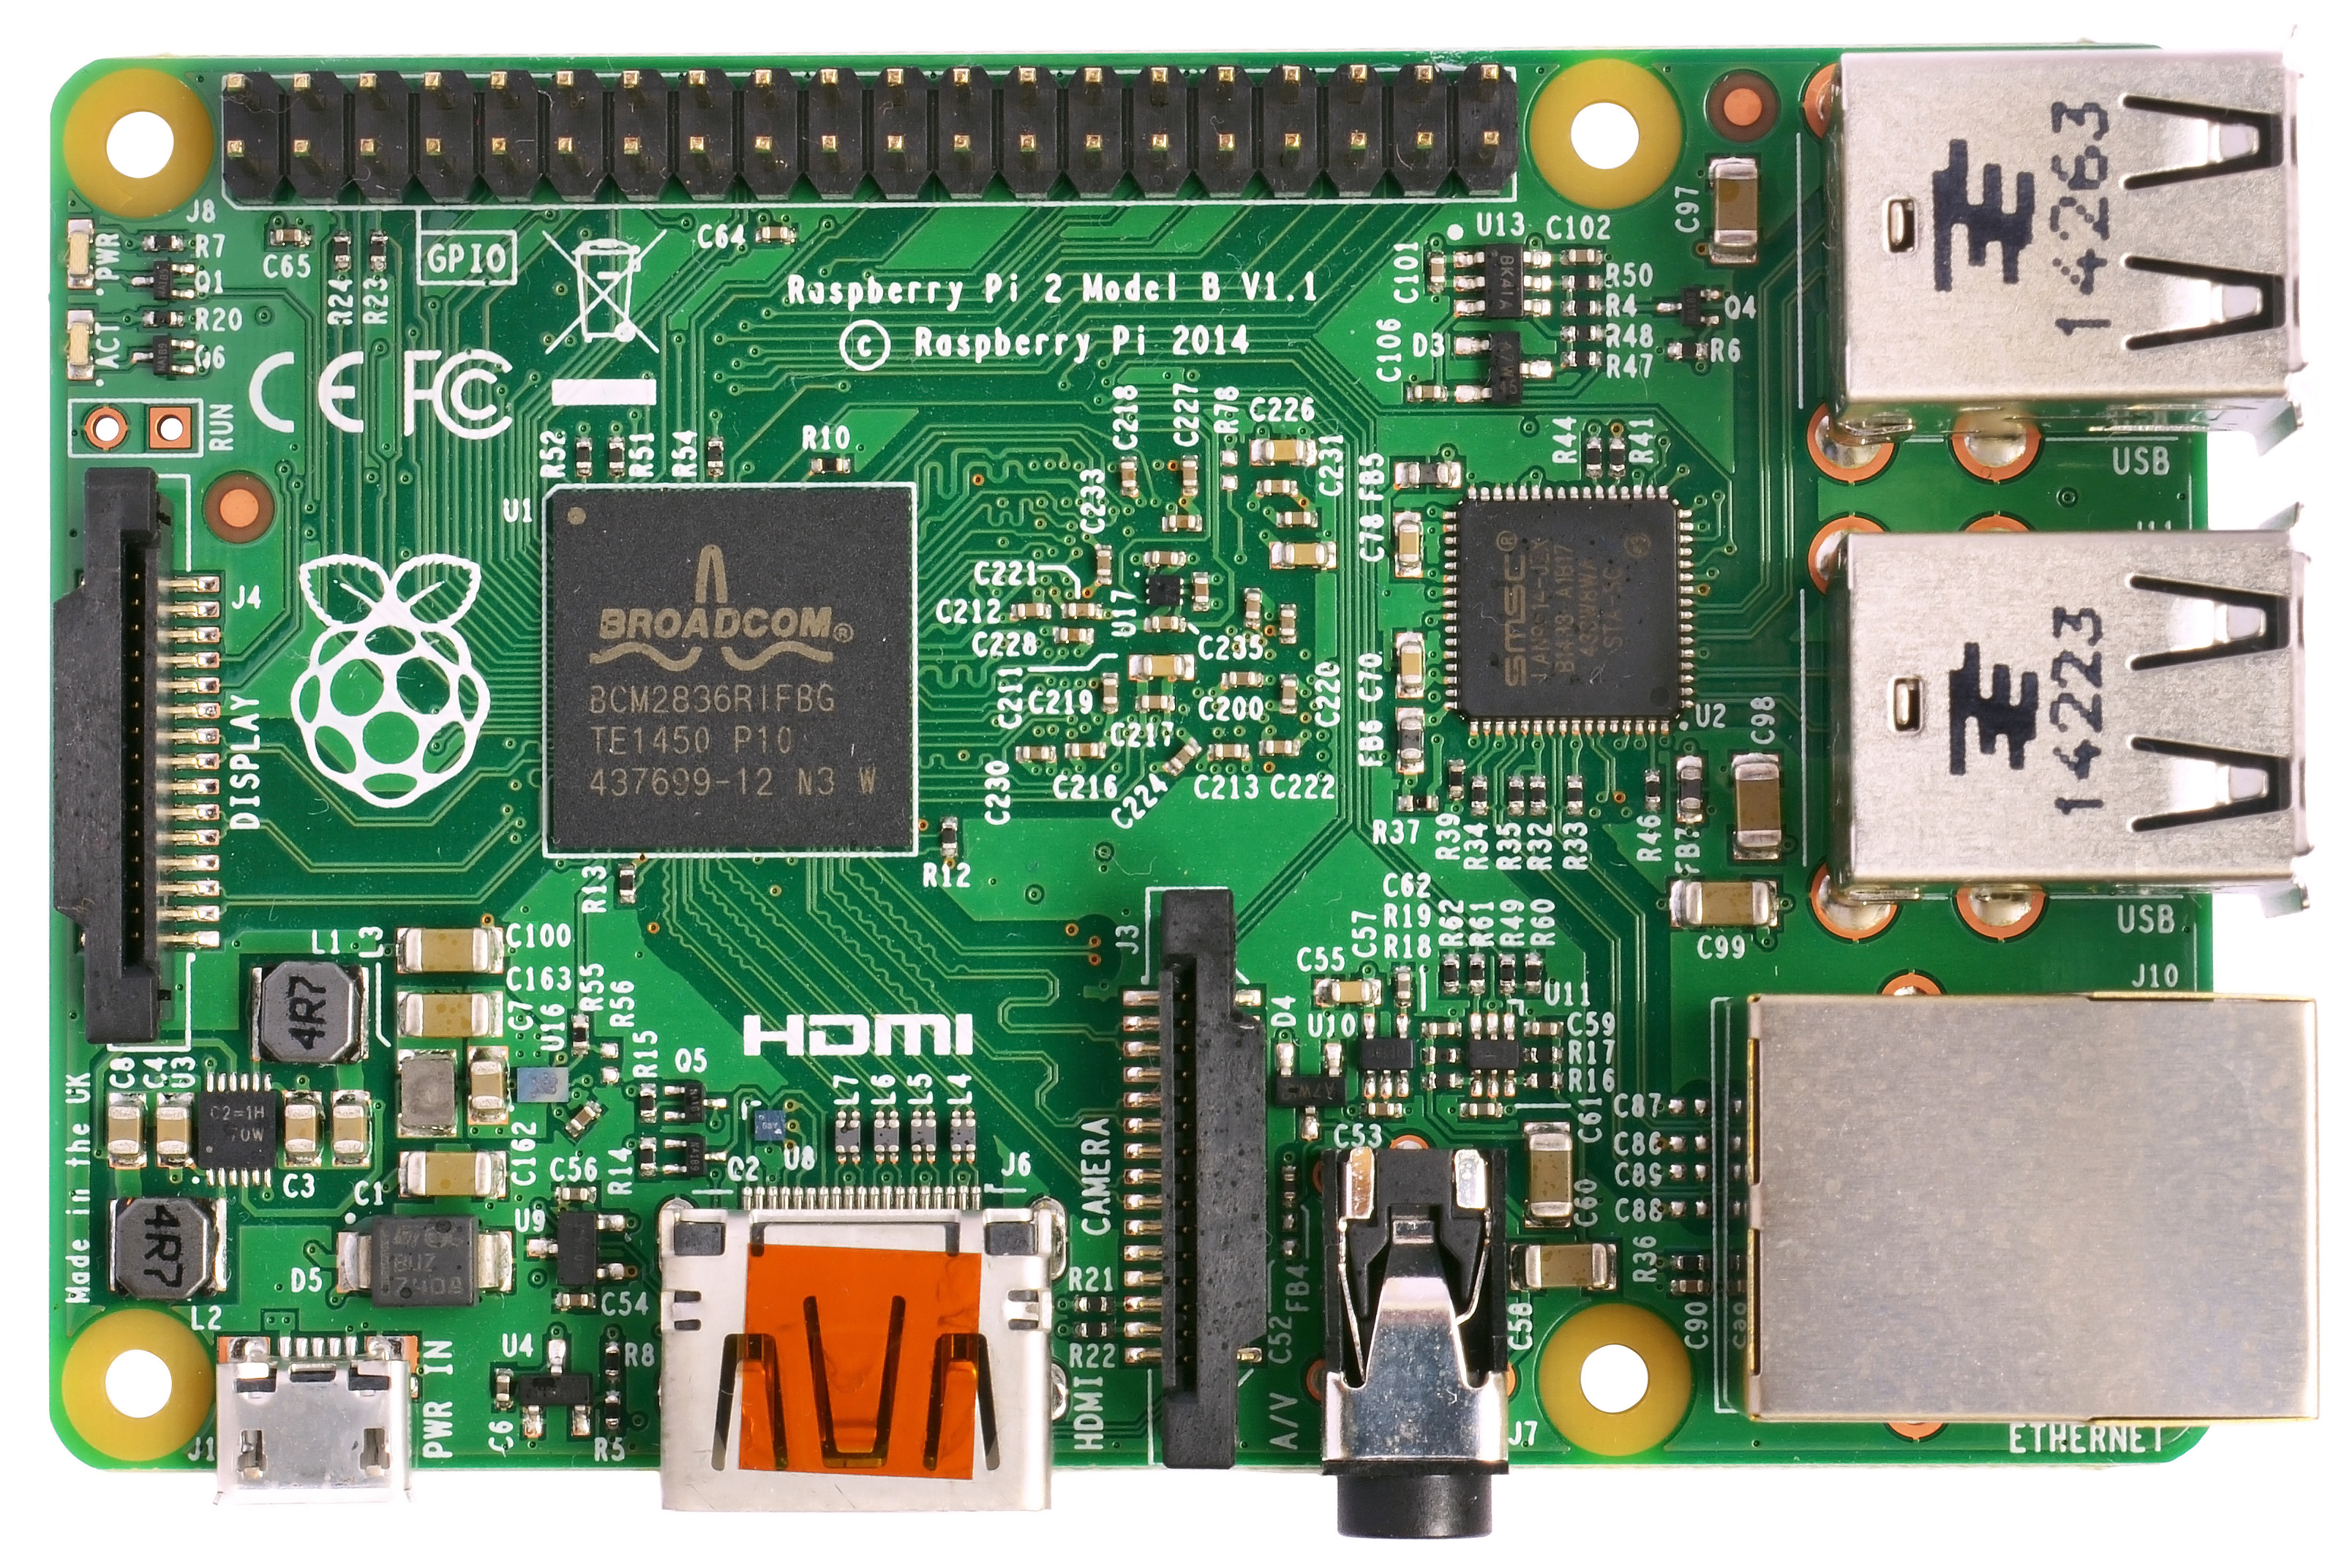
\includegraphics[width=10cm,height=10cm,keepaspectratio]{RPi2}
		\caption{Top portion of Raspberry Pi 2 Model B}
	\end{figure}
\end{frame}

\begin{frame}{OS}
	\begin{itemize}
		\item OS is installed on a micro SD card
		\item Raspbian is optimized OS for RPi
		\item Available at \url{https://www.raspbian.org/}
		\item Micro SD cards with pre-installed OS are also available
		\item Installation
		\begin{itemize}
			\item Format the card
			\item Install NOOBS
			\item Choose Raspbian
			\item Install
		\end{itemize} 
	\end{itemize}
\end{frame}
\begin{frame}{Python on RPi}
	\begin{itemize}
		\item Used to program to access pins and process
		\item Can use any language!
		\item $C$ and $C++$ requires a compiler called \textbf{gcc} which is pre-installed
		\item Python interpreter is also pre-installed
		\item We shall use Python $3$ instead of Python $2$ here because most packages for RPi usage are written in Python $3$
	\end{itemize}
\end{frame}

\begin{frame}{Writing python code}
	\begin{itemize}
		\item Python programming Environments
		\begin{itemize}
			\item IDE
			\begin{itemize}
				\item Combines the facilities of interpreter and text editor
				\item Default IDE is IDLE
				\item Invoke: Menu $\rightarrow$ Programming $\rightarrow$ Python
				\item Select Python $3$
			\end{itemize}
			\item Text-editor and interpreter separately
			\begin{itemize}
				\item Use \textbf{nano} to write code (ex: hello.py)
				\item Execute the program by typing \textbf{python3 hello.py}
			\end{itemize}
		\end{itemize}
	\end{itemize}
\end{frame}

\begin{frame}{GPIO configuration}
	\begin{figure}
		\centering
		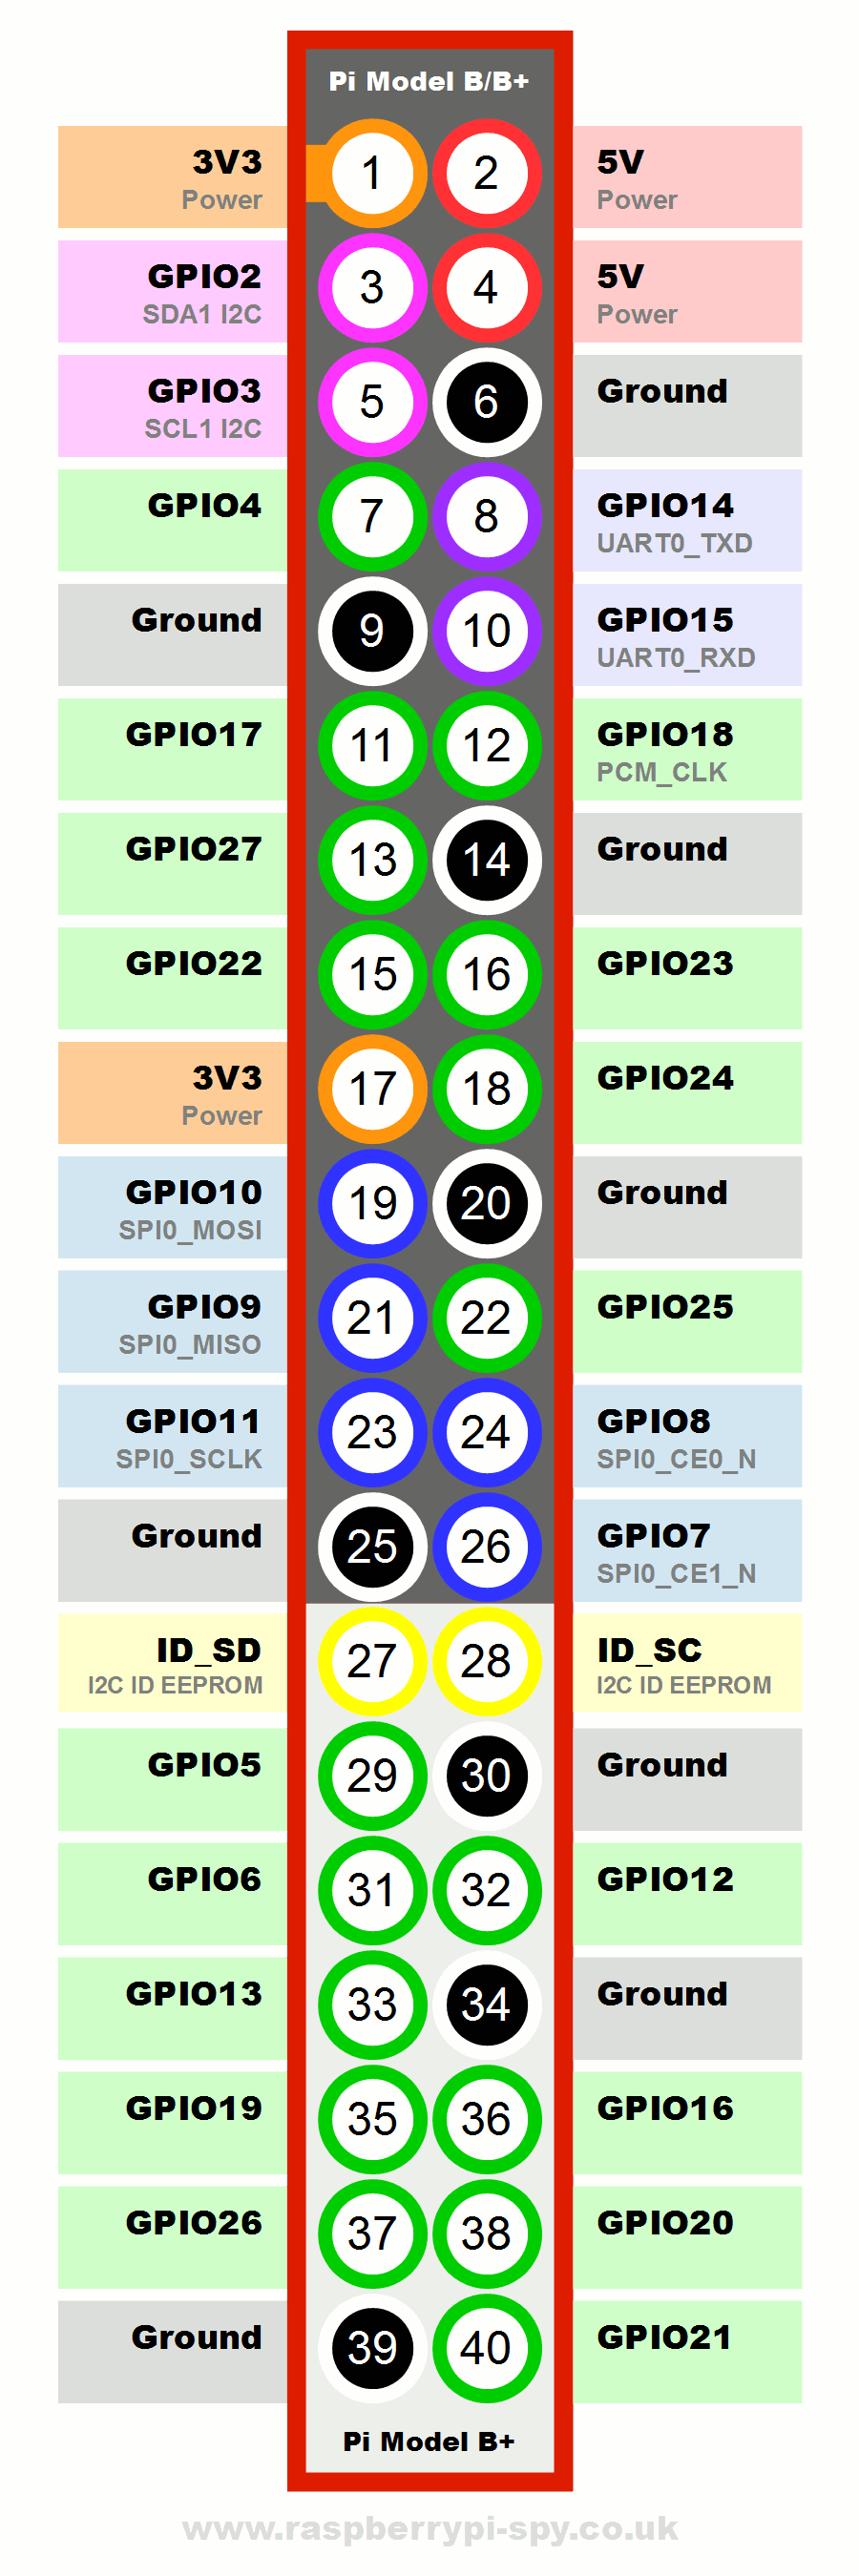
\includegraphics[width=4cm,height=7cm,keepaspectratio]{gpio}
	\end{figure}
\end{frame}

\begin{frame}{GPIO}
	\begin{itemize}
		\item Dedicated power and ground pins
		\begin{itemize}
			\item $3.3V (1,17)$
			\item $5V (2.4)$
			\item GND $(6,9,14,20,30,39)$
		\end{itemize}
		\item GPIO = General Purpose Input Output
		\item Make pins \textit{input} or \textit{output} pins as per choice
		\item There are two numbering systems
		\begin{itemize}
			\item pin number based on location
			\item Pin number given as GPIO1, GPIO2 etc.
		\end{itemize}
	\end{itemize}
\end{frame}

\begin{frame}{Protocol pins}
	\begin{itemize}
		\item \textbf{I2C}
		\begin{itemize}
			\item Pin no.3 (GPIO2) = SDA1 I2C
			\item Pin No.5 (GPIO3) = SCL1 I2C
			\item Serial communication protocol between two chips relatively closely placed and need to share a clock
			Two wire protocol (SDA = sends Data signal, SCL = sends Clock signal)
		\end{itemize}
		\item If there are several I2C compatible devices, one can connect their SDA and SCL lines together for serial communication between them
	\end{itemize}
\end{frame}

\begin{frame}{Protocol Pins}
	\begin{itemize}
		\item \textbf{SPI}
		\begin{itemize}
			\item 19 (GPIO10) = MOSI (Master Out Slave In)
			\item 21 (GPIO9) = MISO (Master In Slave Out)
			\item 23 (GPIO11) = SCLK (S Clock)
			\item 24 (GPIO8) = CE01 (Chip Enable)
			\item 26 (GPIO7) = CE02 (Chip Enable)
		\end{itemize}
	\end{itemize}
\end{frame}


\end{document}